%====================================================================================
\section[Bién Público]{Bienes Públicos y Eficiencia Económica}
%====================================================================================

\begin{frame}{Bienes Públicos y Eficiencia Económica}
	\begin{itemize}
		\item Cuando los bs. Públicos se otorgan gratuitamente, no hay un indicador (precios) que diga si se está ofreciendo una cantidad apropiada o no. 
		\item Tampoco se cuenta con un indicador de la valoración individual.
		\item Ese rol lo cumplen los precios en bs. Privados.
		\item Origen del problema: los bs. Públicos se consumen “en común”, mientras el mercado piensa en la toma de decisiones individuales.
		\item La indivisibilidad de los bs. Públicos dificulta determinar la cantidad en que la sociedad debe producir dichos bienes.
	\end{itemize}
\end{frame}
%------------------------------------------------
\begin{frame}{Bienes Públicos y Eficiencia Económica}
	Se tiene dos consumidores ($A$ y $B$) y dos bienes ( 1 = bien público; 2= bien privado)
		\begin{center}
			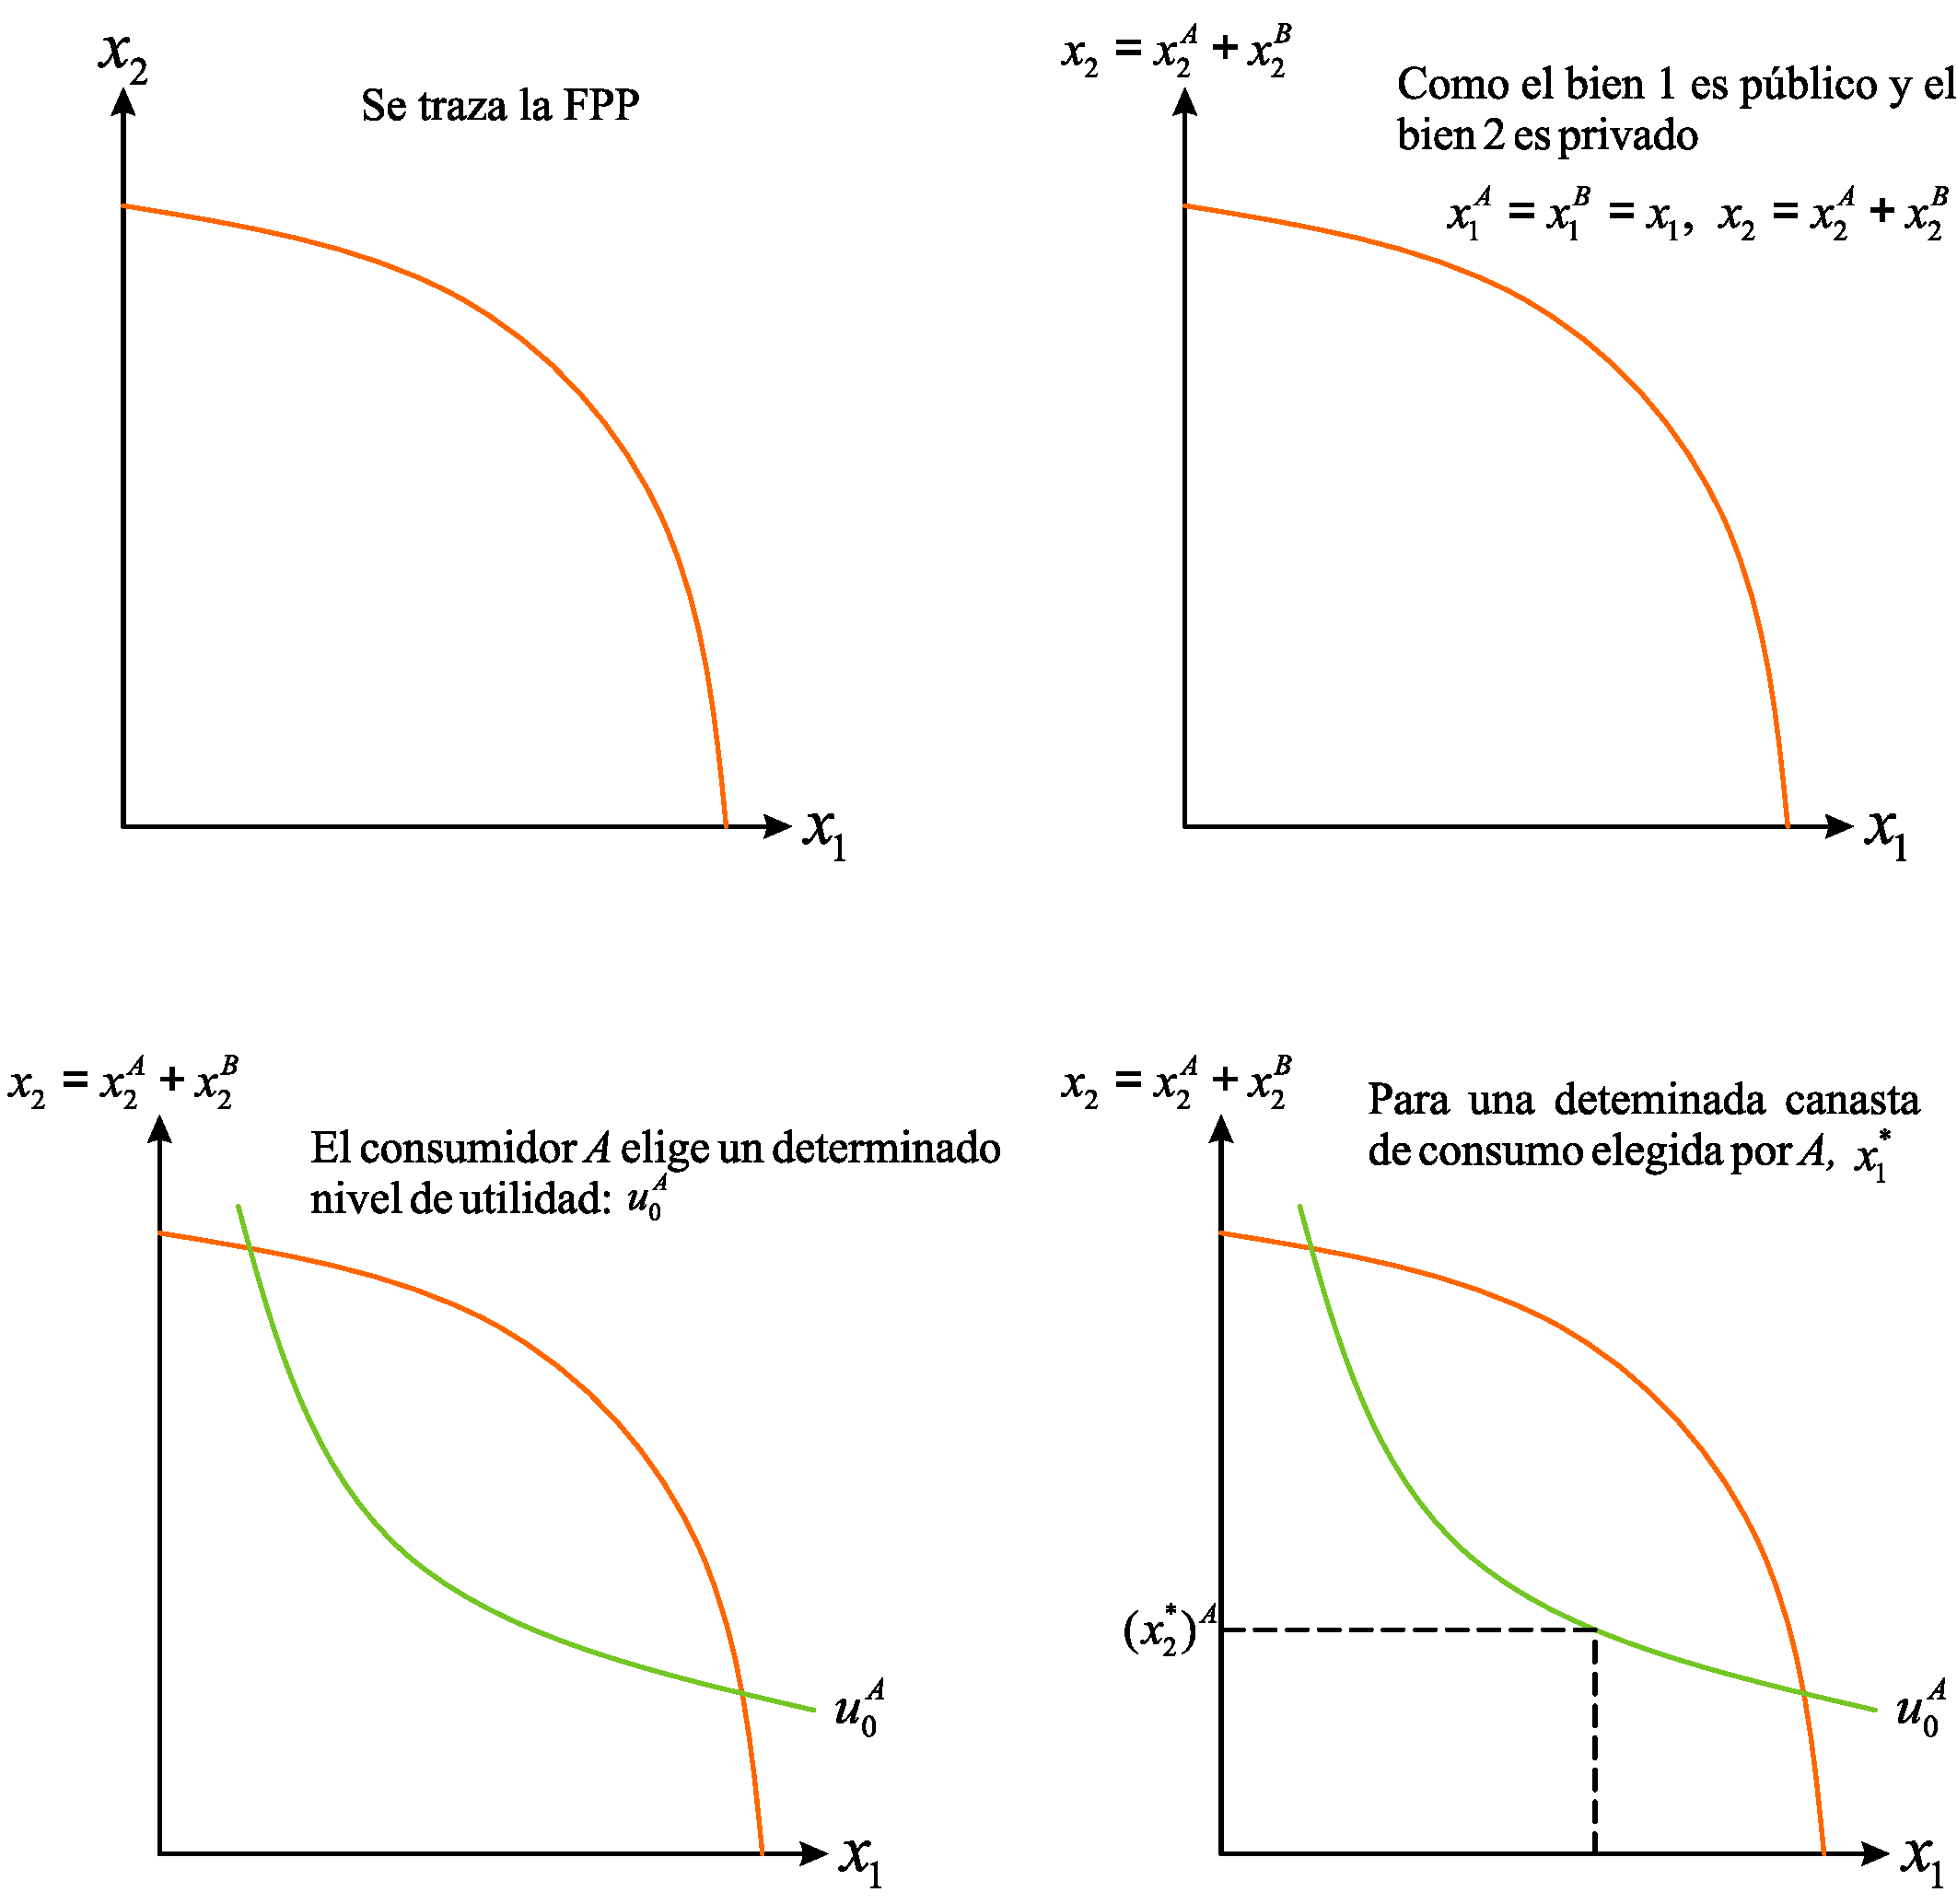
\includegraphics[width = 0.65\linewidth]{figures/fig_02.pdf}
		\end{center}
\end{frame}
%------------------------------------------------
\begin{frame}{Bienes Públicos y Eficiencia Económica}
	\begin{center}
		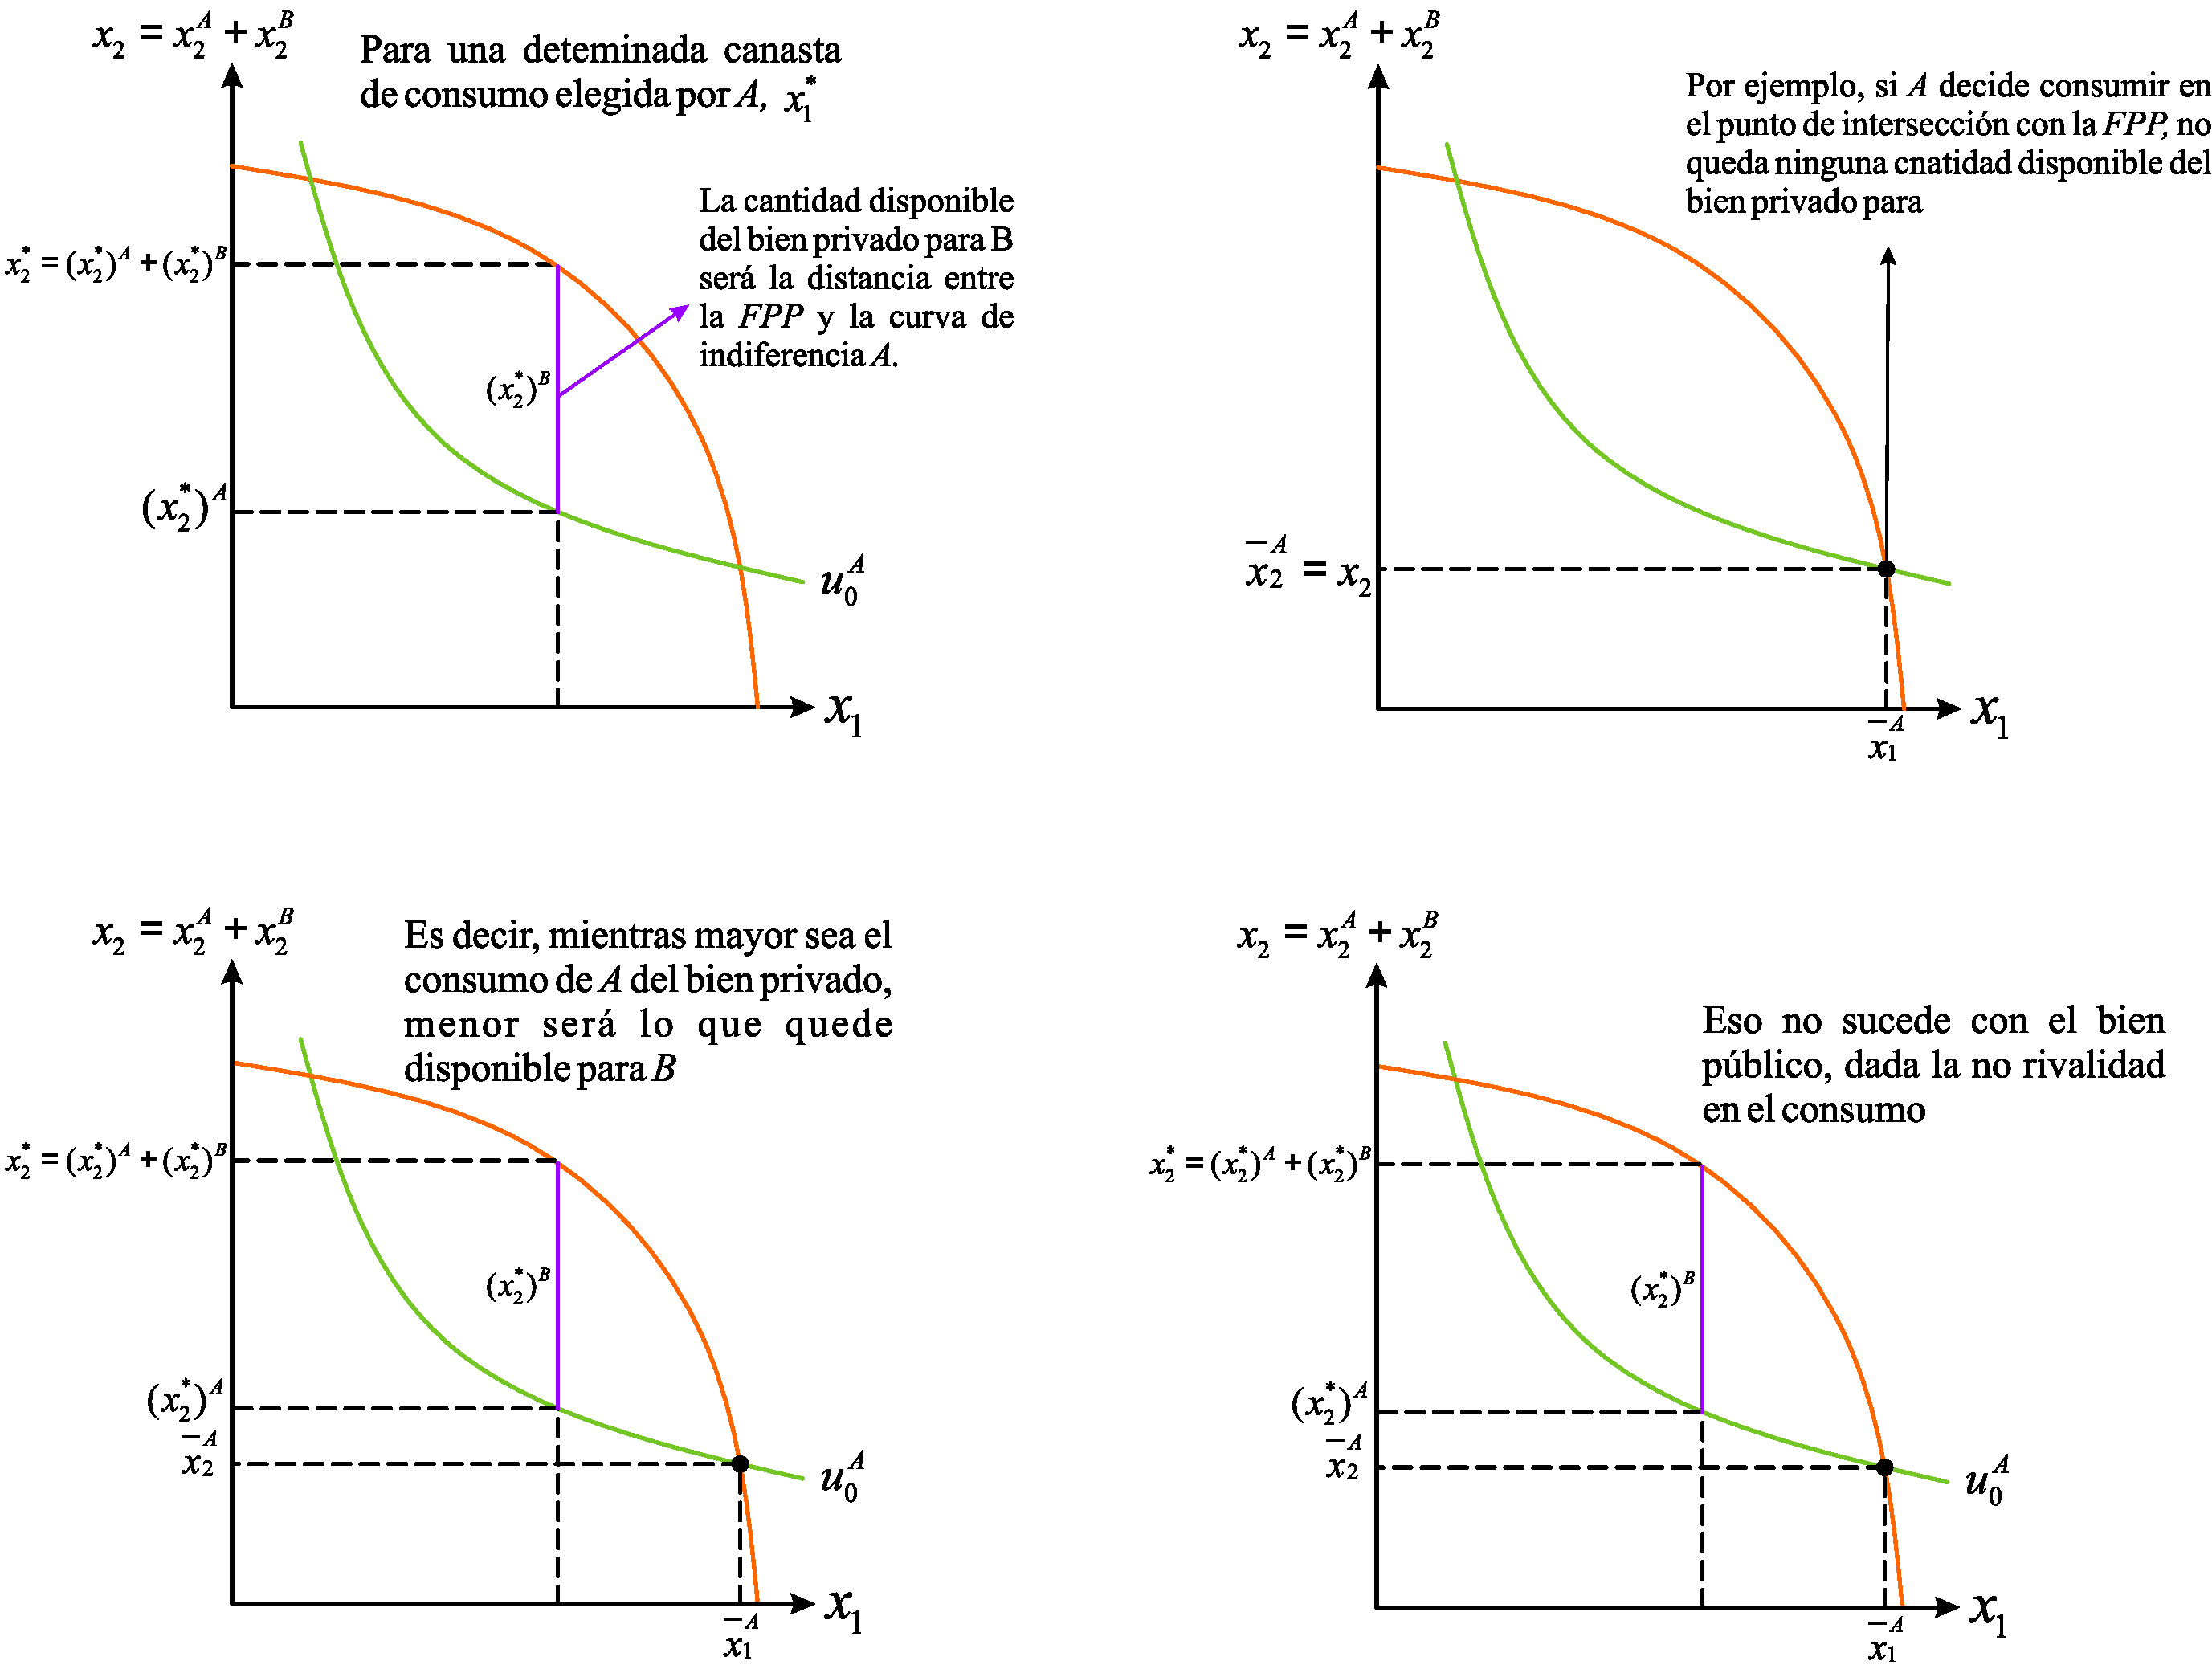
\includegraphics[width = 0.98\linewidth]{figures/fig_03.pdf}
	\end{center}
\end{frame}
%------------------------------------------------
\begin{frame}{Bienes Públicos y Eficiencia Económica}
	\begin{center}
		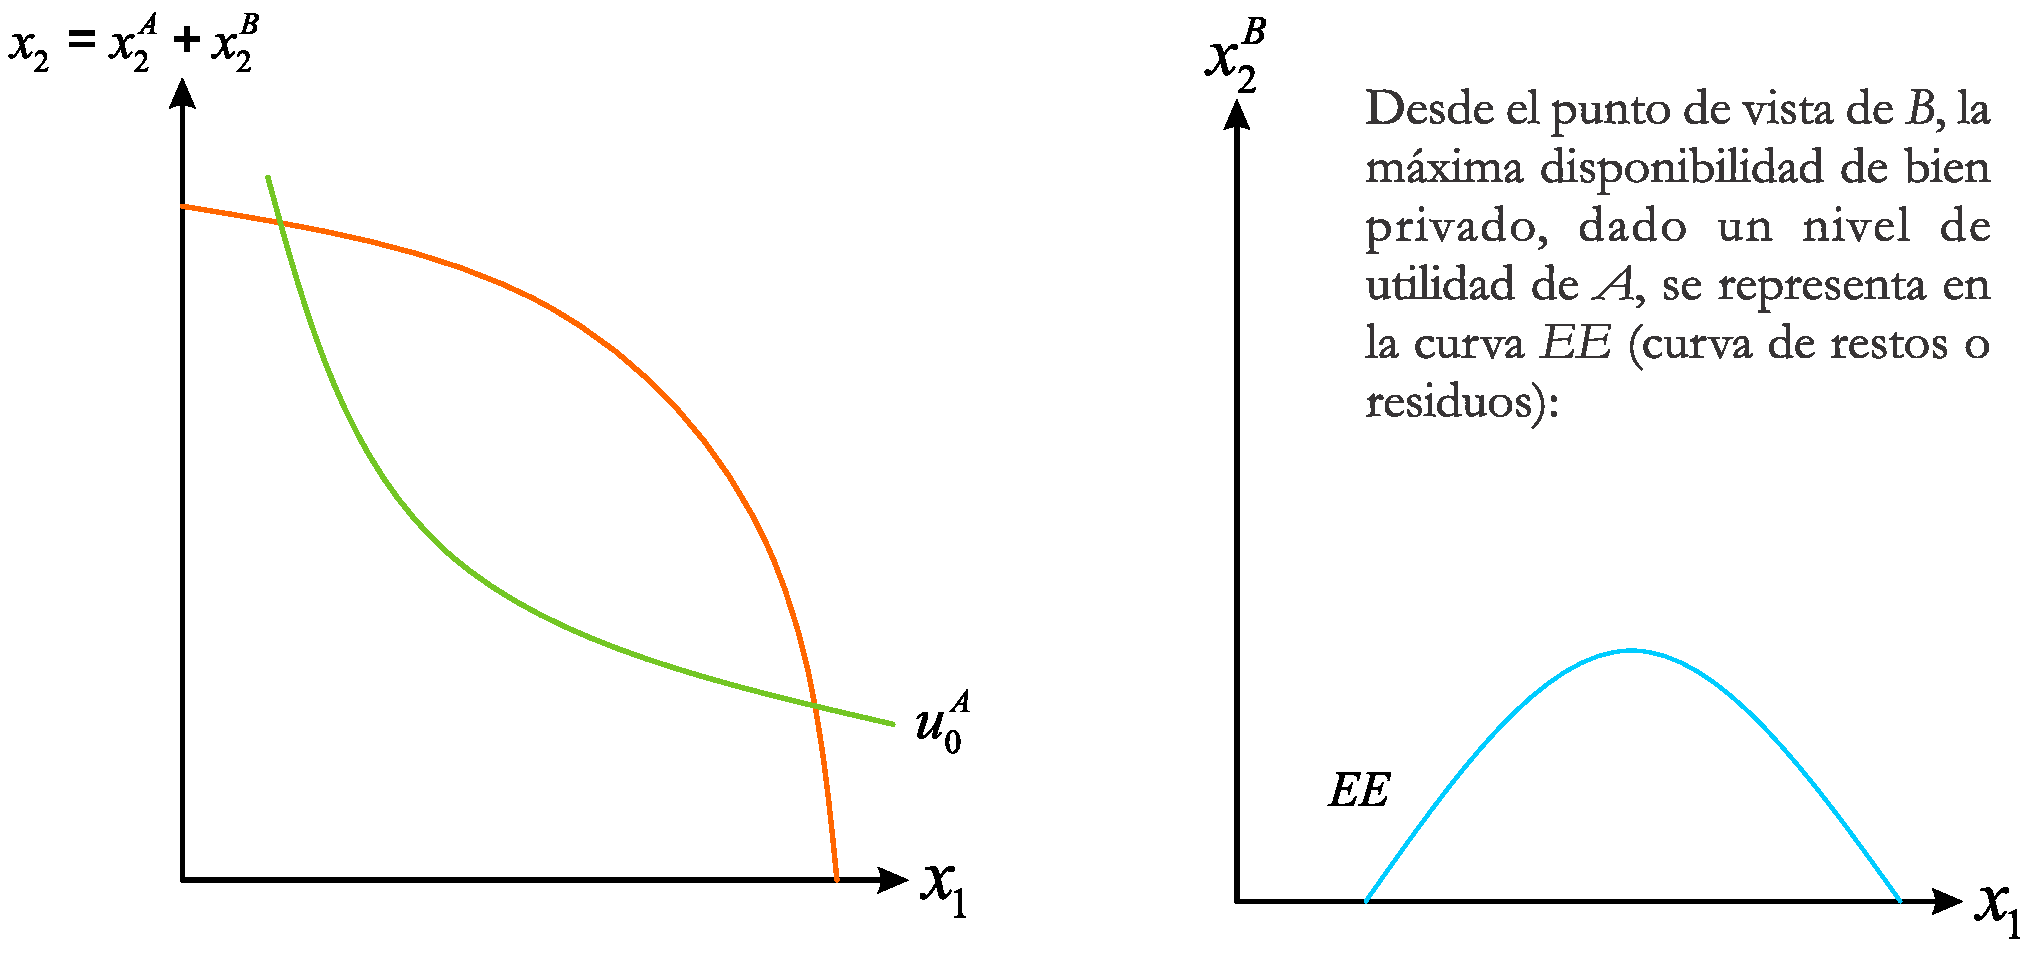
\includegraphics[width = 1\linewidth]{figures/fig_04.pdf}
	\end{center}
\end{frame}
%------------------------------------------------
\begin{frame}{Bienes Públicos y Eficiencia Económica}
	\begin{center}
		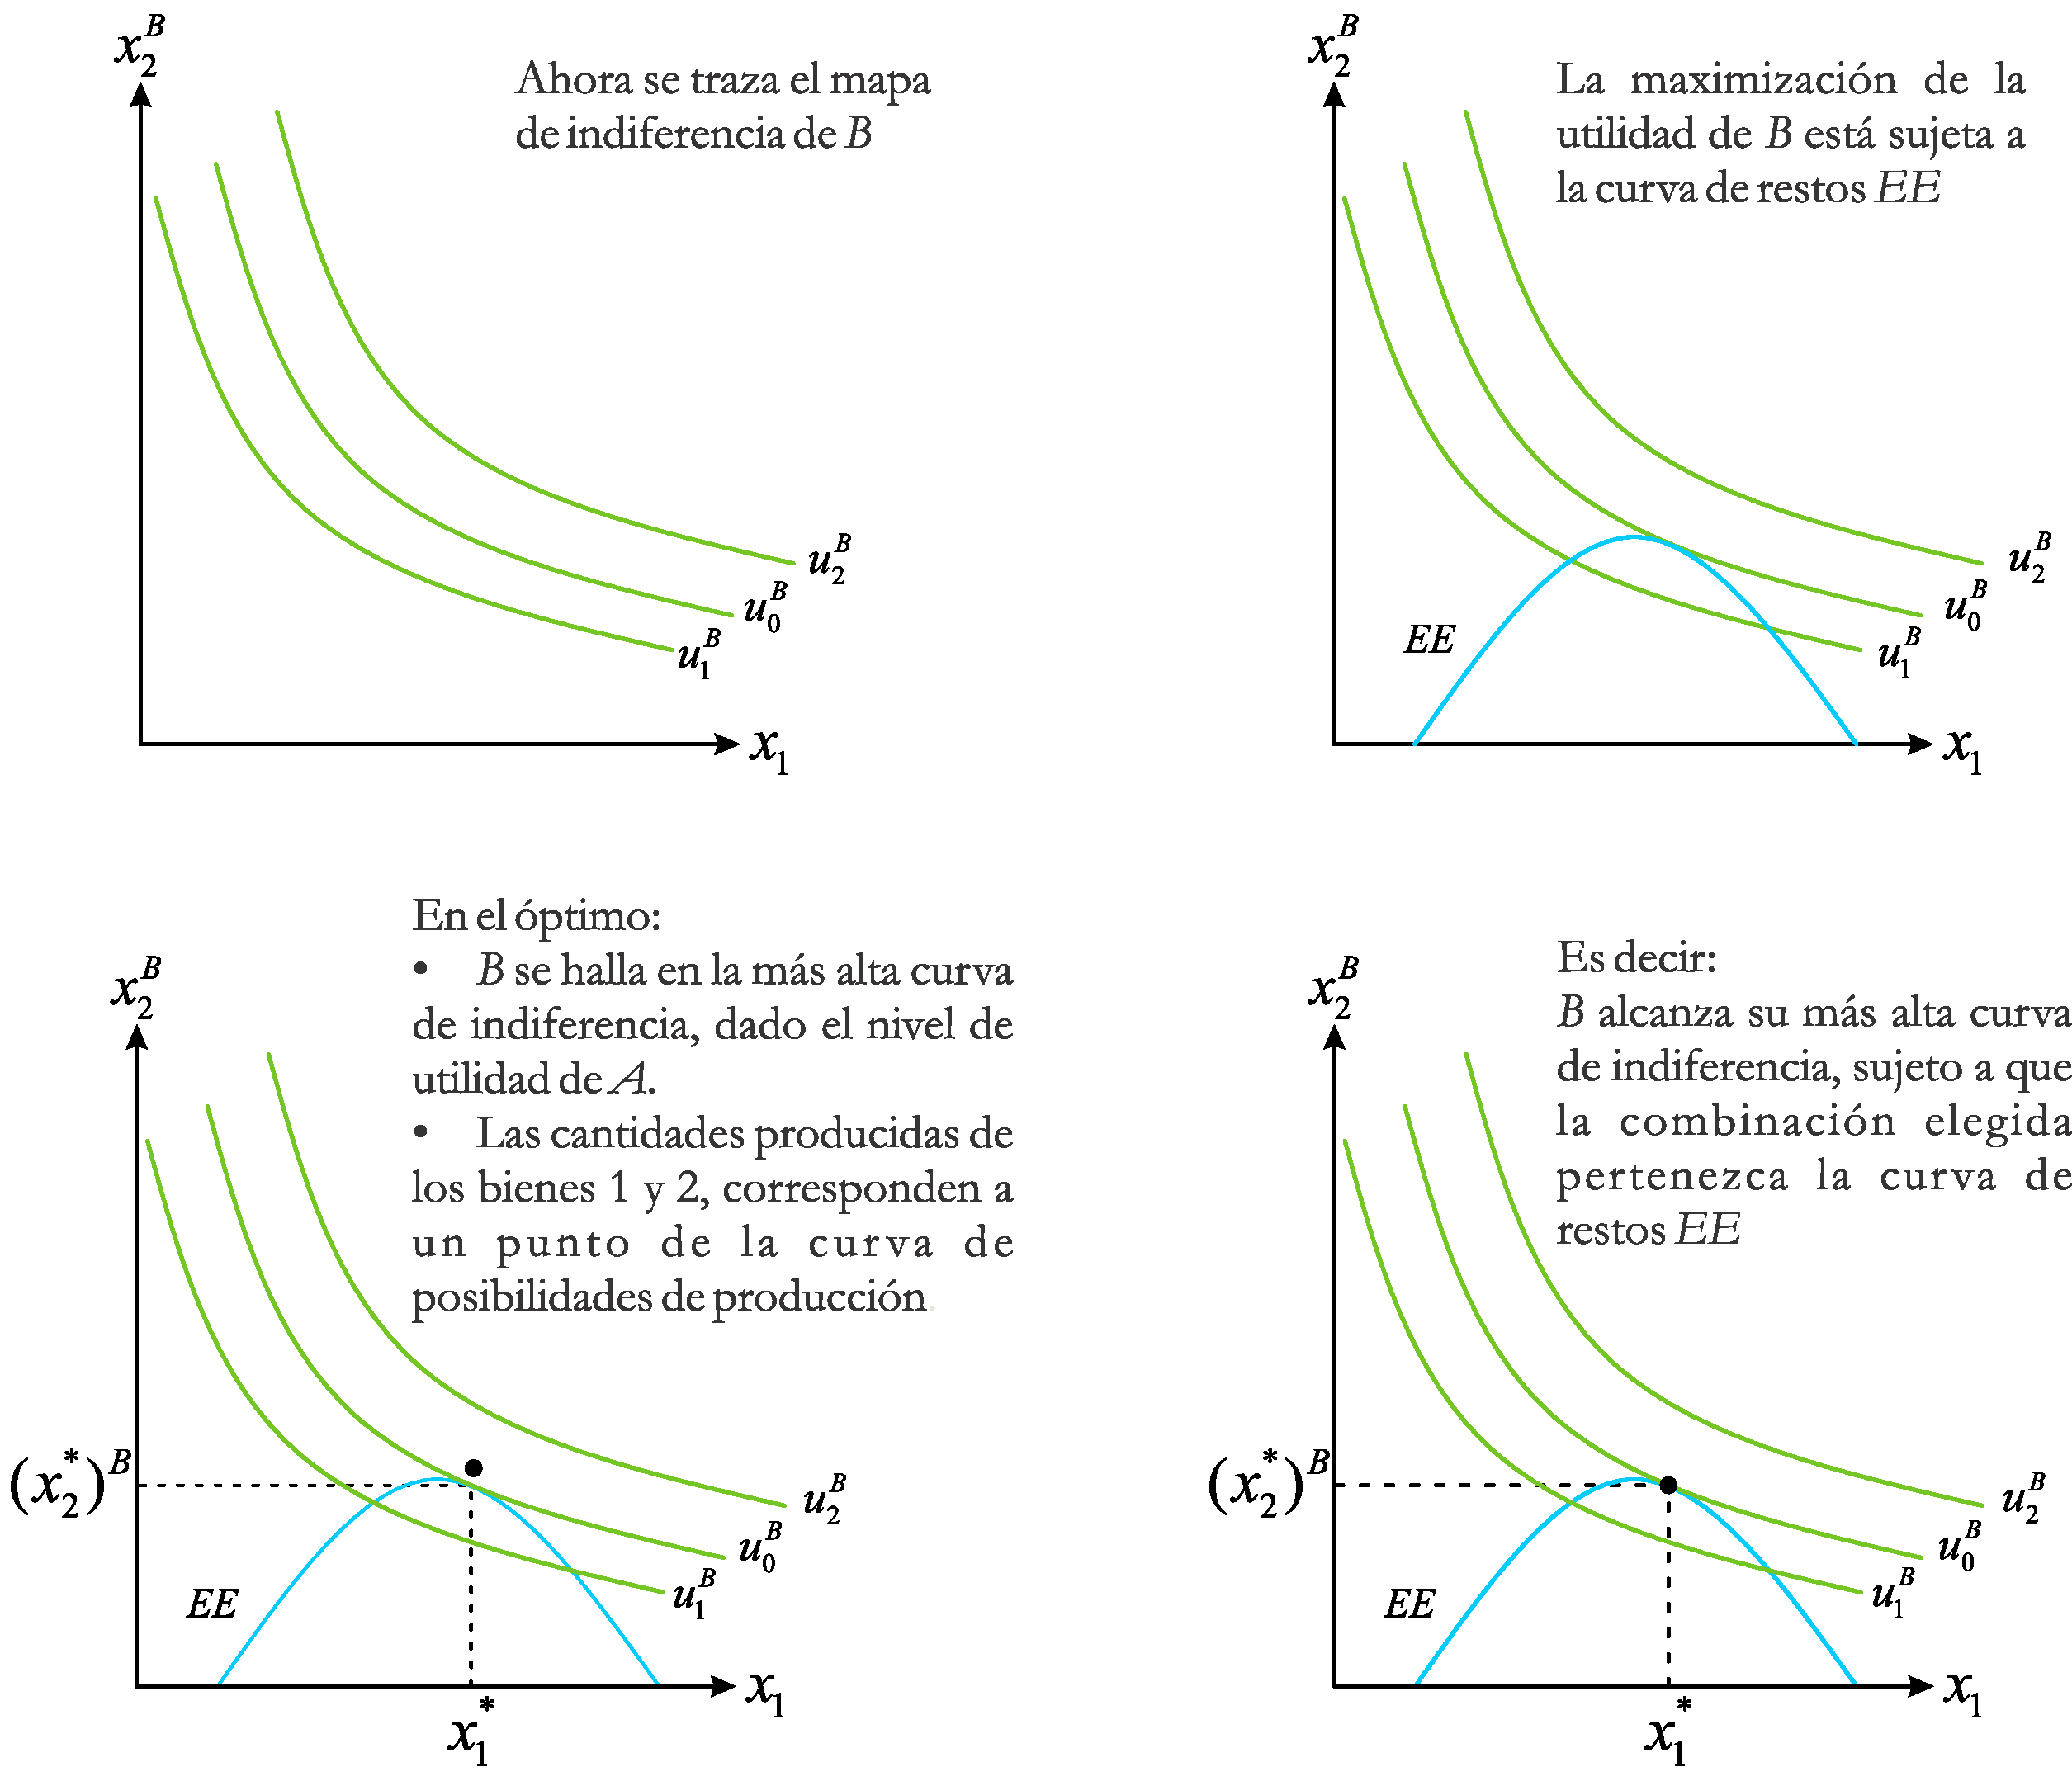
\includegraphics[width = 0.85\linewidth]{figures/fig_05.pdf}
	\end{center}
\end{frame}
%------------------------------------------------
\begin{frame}{Bienes Públicos y Eficiencia Económica}
	\begin{center}
		\hspace{-0.5cm} 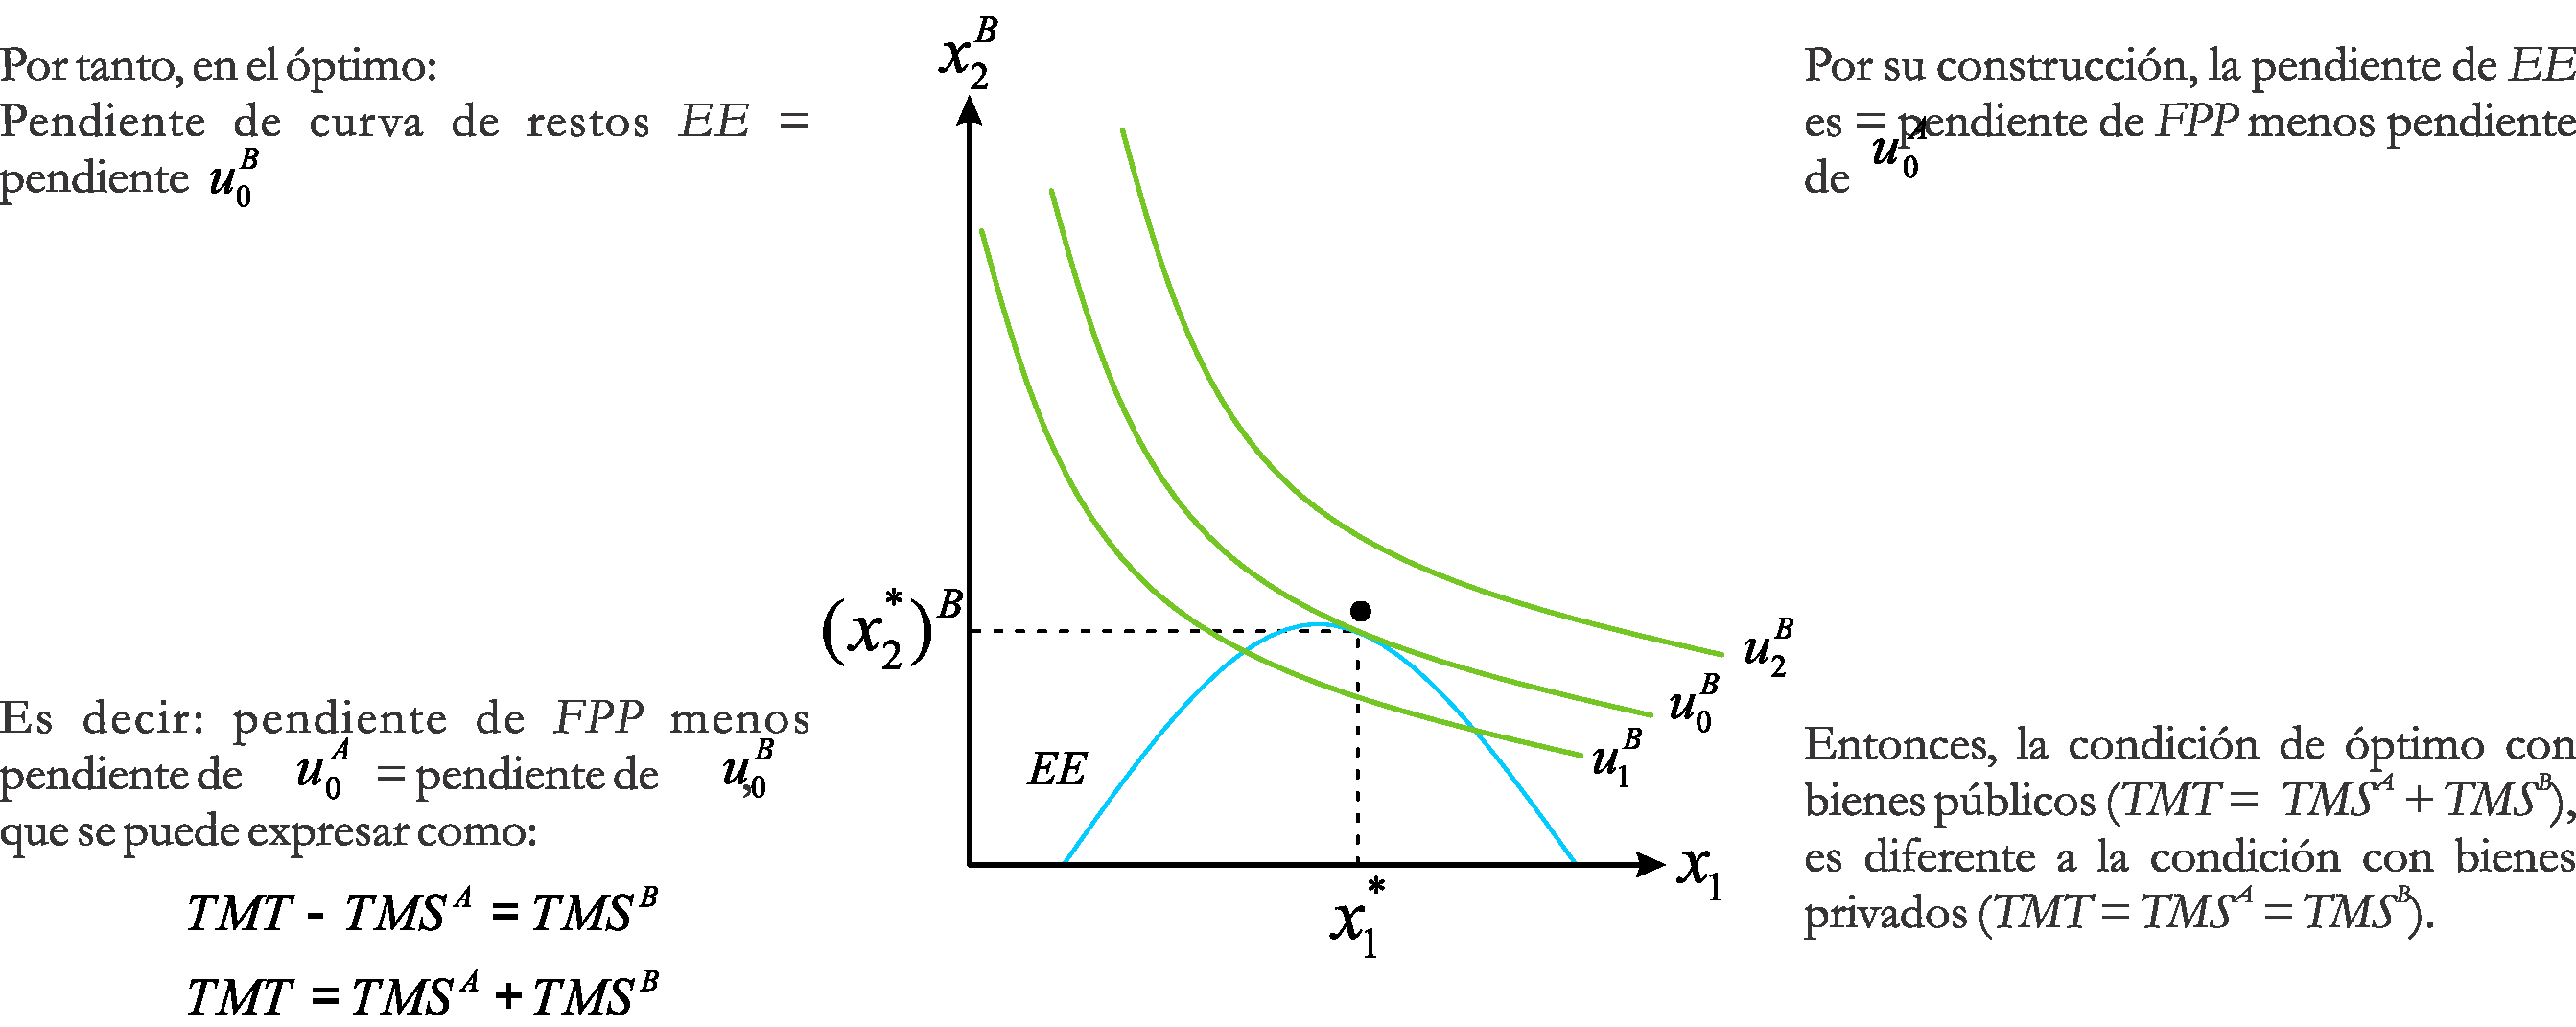
\includegraphics[width = 1.05\linewidth]{figures/fig_06.pdf}
	\end{center}
\end{frame}
%------------------------------------------------
\begin{frame}{Resumen gráfico}
	\begin{center}
		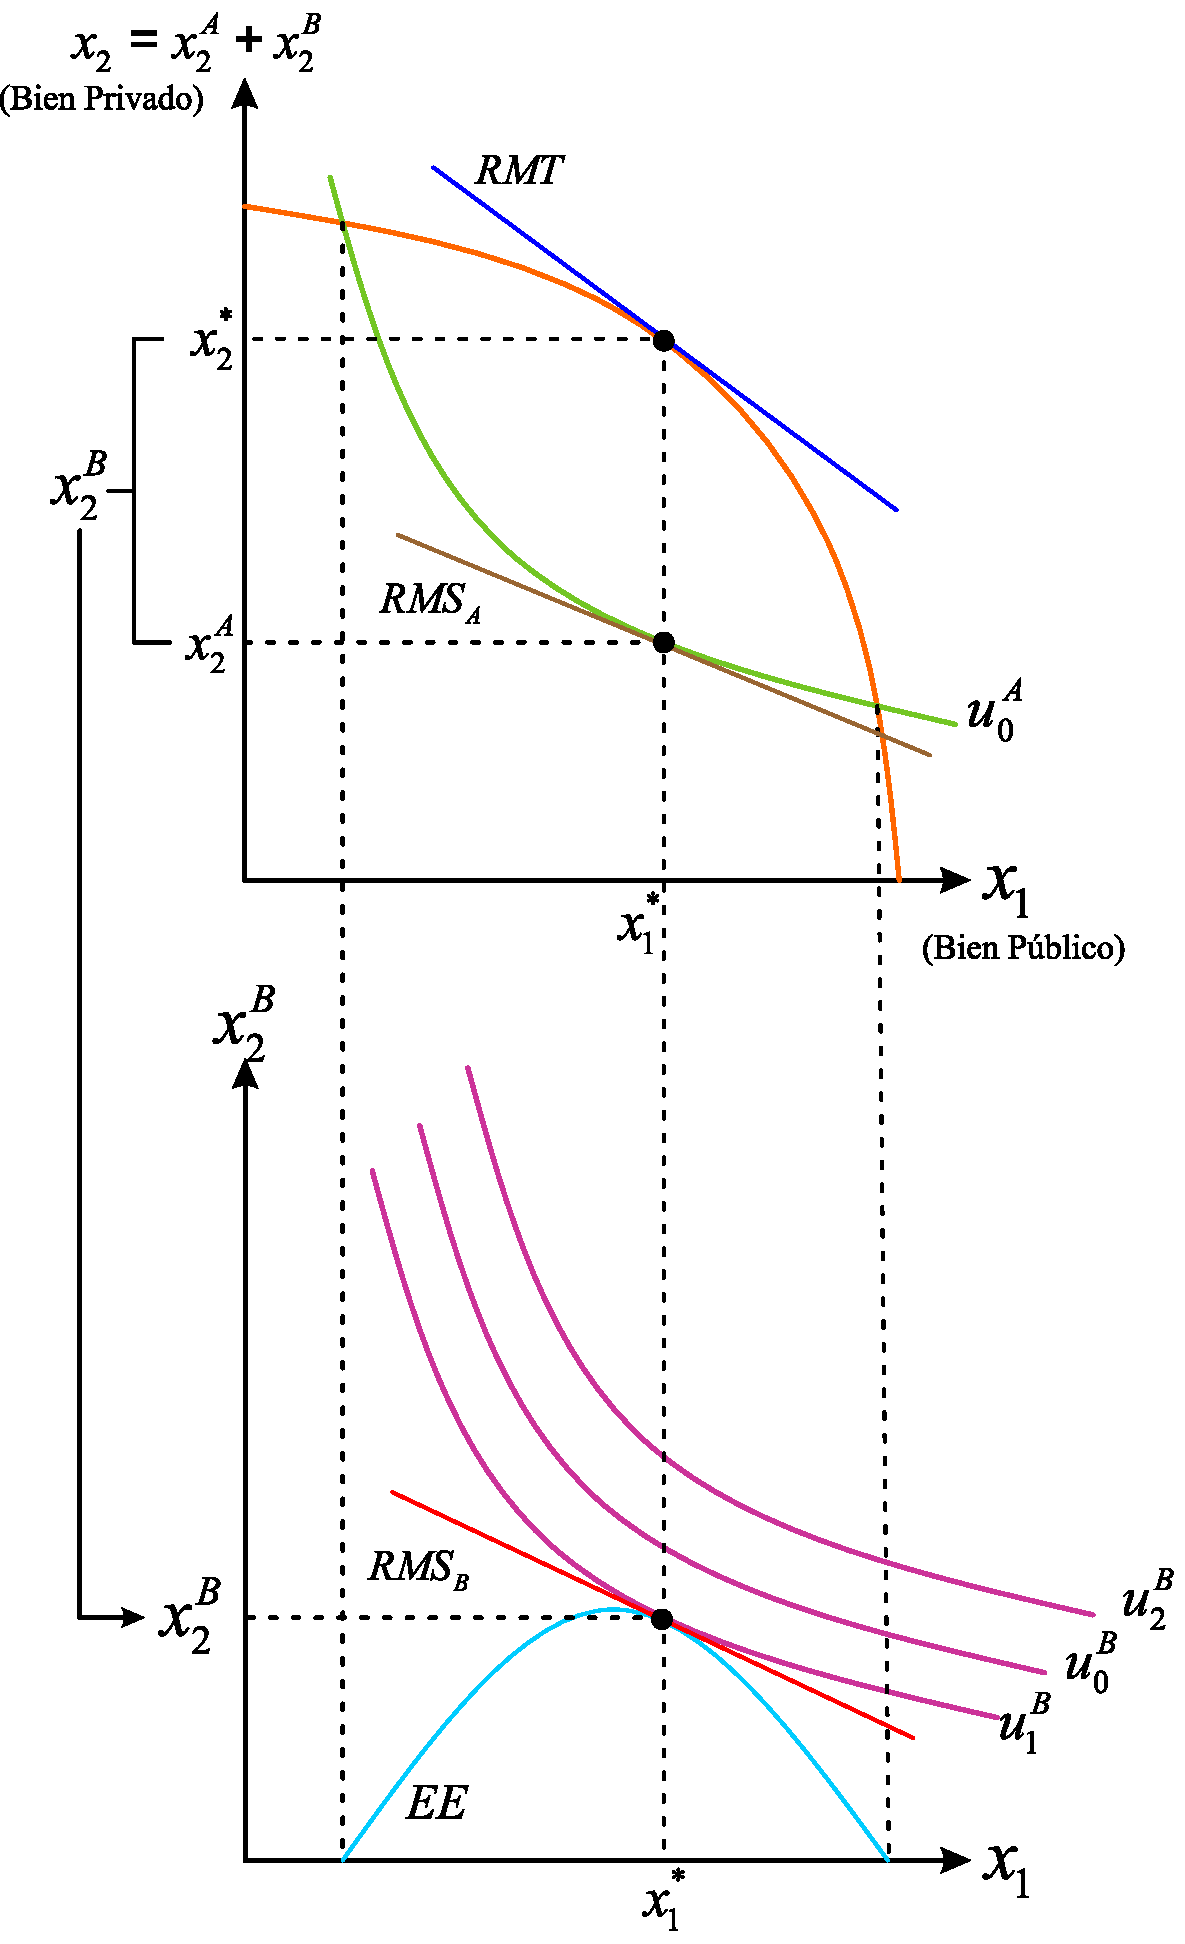
\includegraphics[width = 0.45\linewidth]{figures/fig_07.pdf}
	\end{center}
\end{frame}
%------------------------------------------------
\begin{frame}{Bienes Públicos y Eficiencia Económica}
	¿Por qué es la diferencia?
		\begin{itemize}
			\item Con bienes privados:
				\begin{itemize}
					\item Una unidad adicional de bien privado va al consumidor $A$ o al consumidor $B$.
					\item La eficiencia es alcanzada cuando ambos consumidores tienen el mismo valor marginal de dicha unidad adicional.
				\end{itemize}
			\item Con bienes públicos:
				\begin{itemize}
					\item Una unidad adicional de bien público beneficia a ambos consumidores
					\item Por ello los beneficios marginales deben ser sumados.
				\end{itemize}
		\end{itemize}
\end{frame}